\vspace{0.5cm}
\begin{figure}[H]
  \centering
  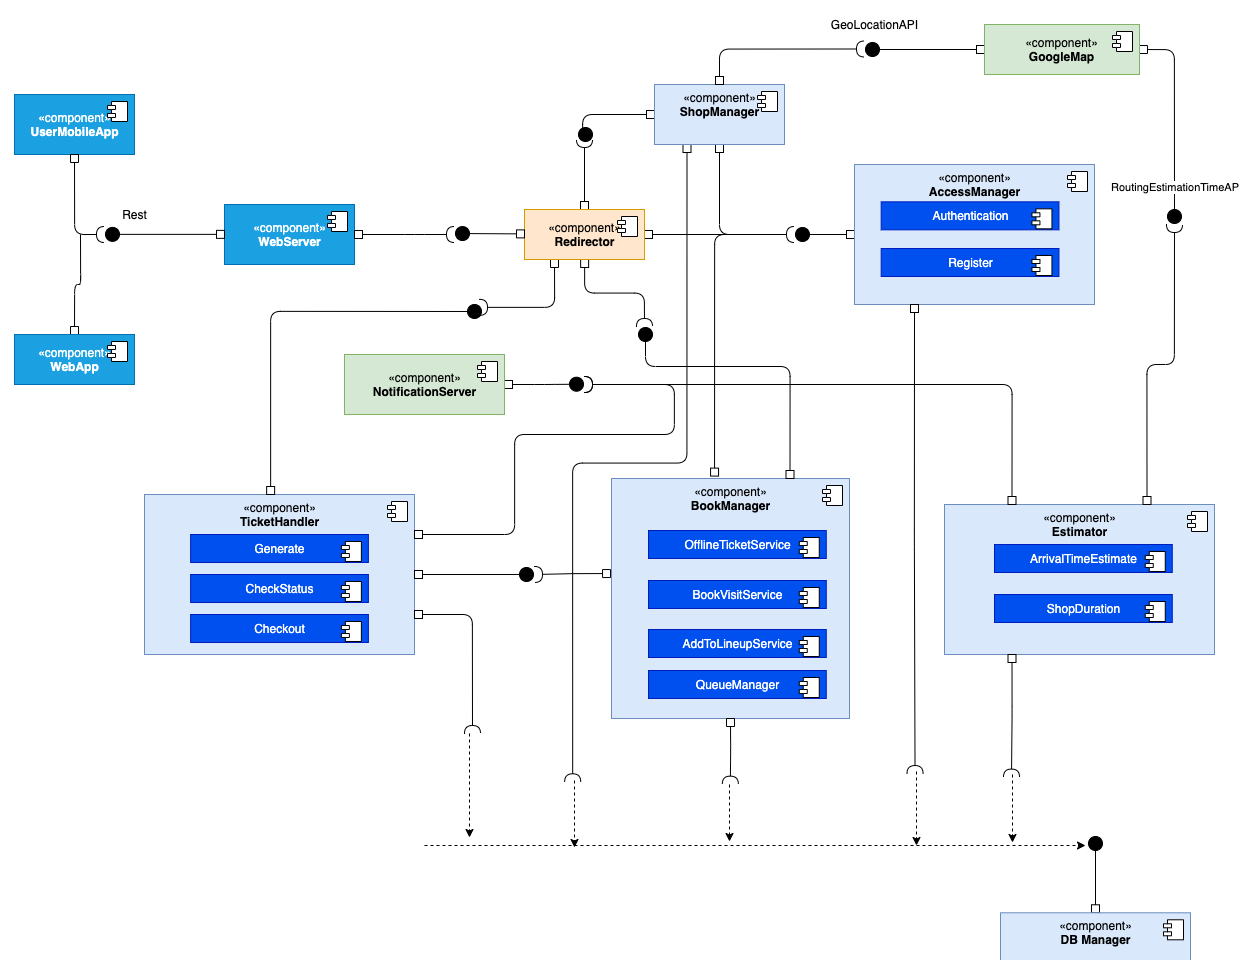
\includegraphics[width=0.9\textheight,angle =90 ,keepaspectratio]{images/all/componentview.png}
  \caption{Component Diagram}
\end{figure}
\clearpage

The following component diagram gives a specific view of the system focusing on the representation of the internal structure of the application server, showing how its components interact. The application server contains the business logic of our software. Other elements in the diagram, besides the application server, have been depicted in a simpler way just to show how the communication is structured among these components and the application server.
\begin{itemize}

    \item \textbf{Notification server:} it manages the notification which is used to send to users when its going to be close to be their turn and also their turn to enter the supermarket so it is connected to Estimator component.\\ 
    
    \item \textbf{Booking manager:}  it is divided into some sections:
    \begin{itemize}
        \item \textbf{offlineTicketService:} which it handles and print the tickets in person for whom they do not have smartphone. \\
        \item \textbf{BookVisitService:} which is a booking for those who wants to take a visit in the supermarket and wants to book it before. \\
        \item \textbf{AddToLineupService:} which is a service that users can reserve a slot for themselves at that moment by generating a QR code.\\
        \item \textbf{QueueManager:} This module handles the interactions with queue for each shop.
    \end{itemize}
    
    \item \textbf{Estimator:} this component estimates the time which is divided into two section:
    \begin{itemize}
        \item \textbf{Arrival Time Estimation:} It is going to estimate the time takes from the current location to the store. This component use MapManager which is connected to the google map API. This component ask from notification manager to send a notification to user in proper time.\\
        
        \item \textbf{Shop Duration:} The other section is the shop duration in which it estimates the duration of shopping for each customer thus the system can estimate the time for other users entrance.
        It also connects to google map component to recognize the user's location to notify him if he is nearby the supermarket.
    \end{itemize}
    
    \item \textbf{TicketHandler:} its also divided into some sections:
    \begin{itemize}
        \item \textbf{Generate:} which is about generating QR code for the use of customers to make line-up or booking.\\
        \item \textbf{CheckStatus:} which is anout scanning customers QR code to check if it is valid or not.\\
        \item \textbf{Checkout:} it manages the scanning of QR codes which it results to understanding the checking out of customers and it helps to improve the estimation time for other.
    \end{itemize}
    
    \item \textbf{ShopManager:} this component is related to the shops. users could see the near shops through this components and manager who can add shop into the system and it connects to google map which is a element for them to add the location of the shop. \\
    
    \item \textbf{DBMSManager:} this is the component that allows every other component in the system to interact with the database. The Interface provided by this component contains all useful methods to store, retrieve, update data into the database from different actors. Every internal component of the application server uses some methods of its interface. \\
    
    \item \textbf{Redirector:} this component simply dispatches the requests and calls to methods from the users and the managers to the core of the application server. Every method is redirected to the proper component that can handle it. Also, responses and data sent back pass through this component to reach the applicant.\\
    
    \item \textbf{MapManager:} its connected to google map and make our specific interface and in case if we want to use other map services, we should just change this module.
    
\end{itemize}
The external component of the system is also mentioned:
\begin{itemize}
    \item \textbf{GoogleMap:} this is the component that provides a useful interface used to visualize the map of a specific location requested by the user/managers and estimate time between two points.
\end{itemize}

\subsubsection{Additional specification}
\vspace{0.5cm}
In this project we use fat client for some reasons, first the clients use their cellphones and nowadays cellphones have very good computation power besides, mobiles have their own view that we cannot build in the server and then send to them. usually apps use framework which use webview are slower than normal apps. In addition, we prefer fat client computers over thin clients because fat clients allow easy customization and greater control over installed programs and system configuration. Because output is locally generated, a fat client also enables a more sophisticated graphical user interface and reduced server load.\\
\begin{figure}[H]
  \centering
  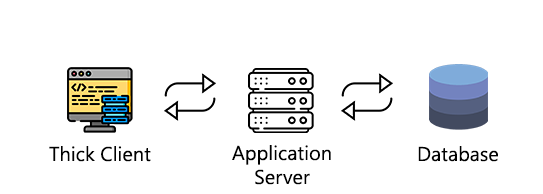
\includegraphics[width=0.8\textwidth,keepaspectratio]{images/all/thickclient.png}
  \caption{Thick(Fat) client}
\end{figure}
In this project, we could duplicate the redirector because as you can see in the component diagram the redirector could be bottleneck of the system. besides, we could have two redirectors at the peak of usage and in the night we could shutdown one of them.\\
We could duplicate the application server then use redirector component as a load balancer between them to guarantee the reliability of the application.
\clearpage